The fitter and background subtraction procedure, introduced in \Cref{sec:fitting_setup,sec:background_subtraction},
have been thoroughly validated in \Cref{sec:MC_validation} -- in simulation.
The real challenge, as usual, is ensuring that the conclusions and results observed in simulation will generalise correctly to real Belle II data.
The key concept of a blinded analysis dictates that one must validate the analysis procedure in control samples or regions -- collections of data that are abundant, well-understood and provide insight to the behaviour of signal in the detector.
In this Section, the discussion about \FEI validation, \piz and $\eta$ veto validation, photon detection efficiency and background modelling will be presented.

\subsection{Calibration of the \texorpdfstring{\FEI}{FEI} algorithm}\label{sec:fei_calibration}

The working principle of \FEI has already been discussed in XXXX
\todo[inline]{xxxx}.
It combines many classifiers which perform reconstructions in various decay chains of the hadronic decays of \B mesons.
Furthermore, the training of the algorithm happens in simulation.
To ensure that the algorithm appropriately acts on data, its performance on Belle II data must be studied, or \textit{calibrated}.
The calibration study is performed on data collected by the Belle~II, for every simulation campaign, and the work is not part of my original work.
Full details of the calibration method are presented in Ref.\cite{Belle-II:2020fst}, but here I will summarise the main details that are relevant to the work of the thesis.

The calibration study uses $B\rightarrow X_{u,c} \ell \nu$ decays, due to branching fraction of almost 20~\% and a clean experimental signature, 
where $X_{u,c}$ denotes an inclusive state originating from the $c$ or $u$ quark, similarly to the $X_s$ notation.
Firstly, in each event, only the highest \FEI probability tag-\B candidate is selected, with loose requirements on Fox-Wolfram moments (see \Cref{sec:fox_wolfram_moments}) and $\Delta E$ to ensure adequate \epem\ra\qqbar suppression.
Next, a high-energy lepton $p_{\ell}^B>1~\gev$ is required in each event.
This lepton candidate is required to originate near the interaction point and its identification information from all sub-detectors is required to be consistent with a lepton.

After the selection, a binned likelihood fit for \Mbc is set up, which contains three binned \PDF{s}: signal $B\rightarrow X_{u,c}\ell\nu$ decays, 
secondary or misidentified leptons, \epem\ra\qqbar events. Here secondary leptons are used to describe leptons that arise in the decay chains of $B$ meson as opposed to the $B\rightarrow X_{u,c}\ell\nu$ decay.
Misidentified leptons are used as a broad term for hadrons whose identification information is consistent with that of either an electron or a muon.
The signal $B\rightarrow X_{u,c}\ell\nu$ \PDF is composed of four sub-\PDF{s}, particularly: $B\rightarrow D\ell\nu$, $B\rightarrow D^*ell\nu$, $B\rightarrow X_u\ell\nu$ and the rest of  $B\rightarrow X_c\ell\nu$ modes.
The fit is performed separately for the following combinations of tag-\B mesons and lepton:
\begin{itemize}
    \item $B^+$ and $e^-$,
    \item $B^+$ and $\mu^-$,
    \item $B^0$ and $e^-$,
    \item $B^0$ and $\mu^-$.
\end{itemize}
This is shown in \Cref{fig:fei_calib}.
\begin{figure}[htbp!]
    \subcaptionbox{\label{fig:fei_calib_bpluseminus}}{
        \clipbox*{{0\width} {0.5\height} {0.5\width} {1\height}}{%
            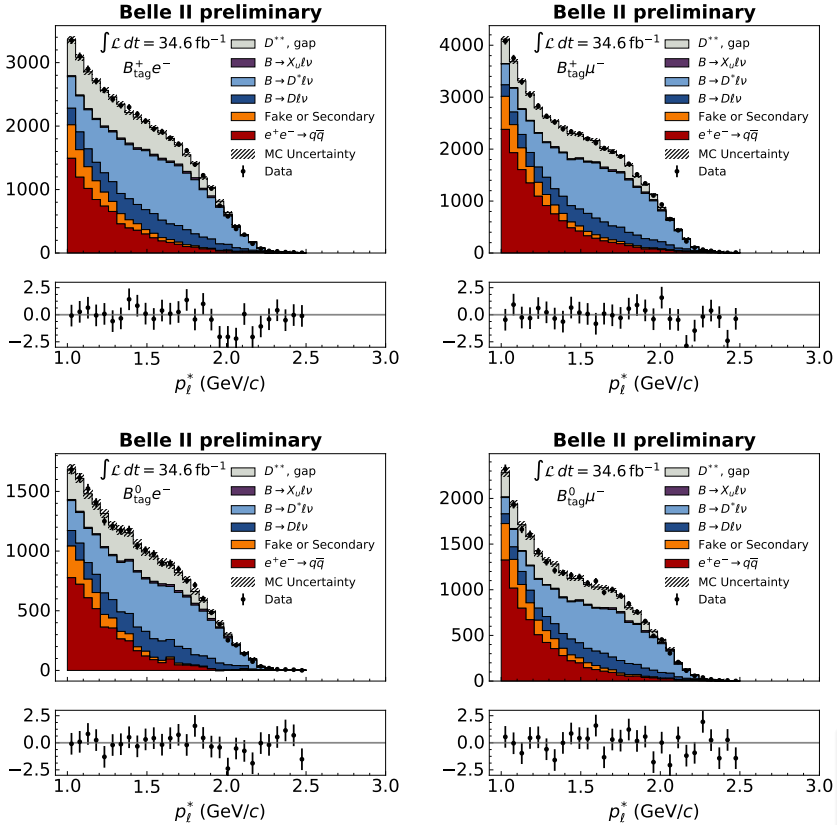
\includegraphics[width=1\textwidth]{figures/data_sim_corrections/tag_calibration.png}
        }
    }
    \subcaptionbox{\label{fig:fei_calib_bplusmuminus}}{
        \clipbox*{{0.5\width} {0.5\height} {1\width} {1\height}}{%
            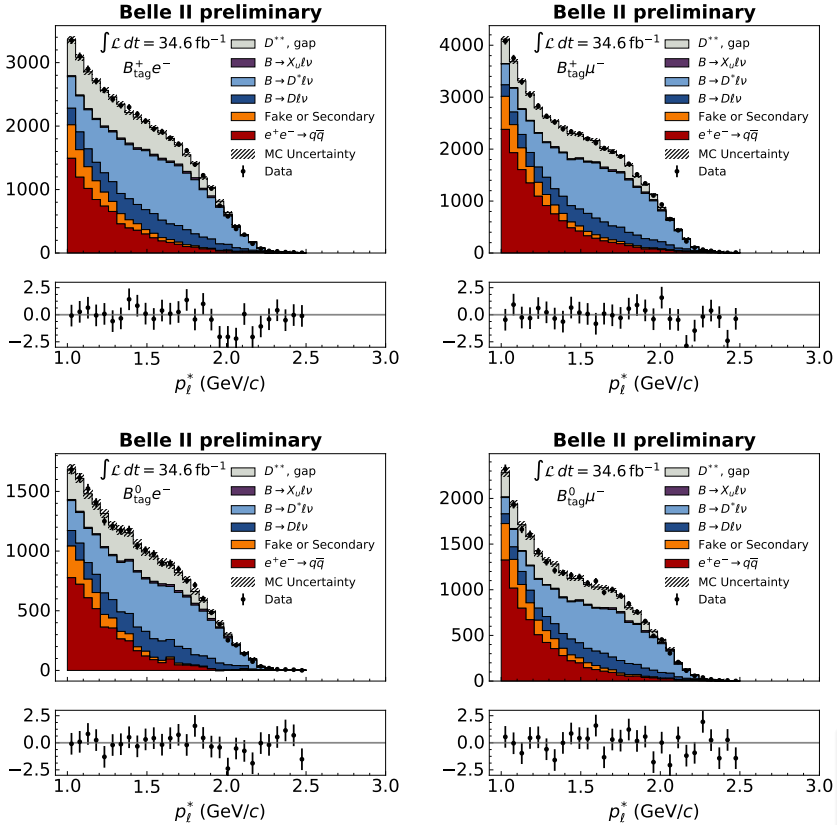
\includegraphics[width=1\textwidth]{figures/data_sim_corrections/tag_calibration.png}
        }
    }
    \subcaptionbox{\label{fig:fei_calib_bzeroeminus}}{
        \clipbox*{{0\width} {0\height} {0.5\width} {0.5\height}}{%
            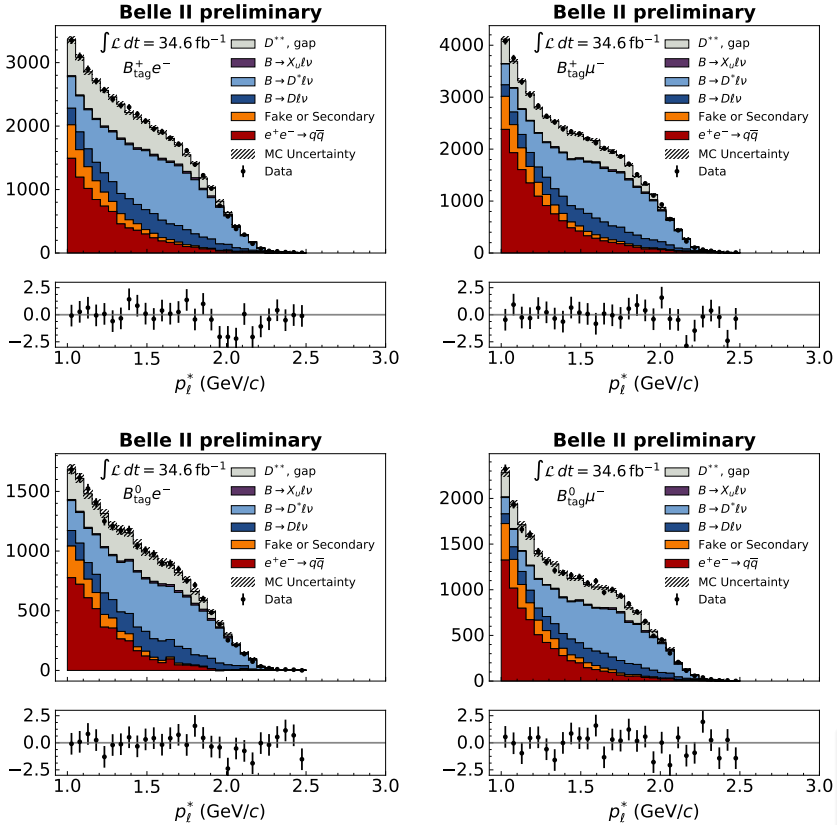
\includegraphics[width=1\textwidth]{figures/data_sim_corrections/tag_calibration.png}
        }
    }
    \subcaptionbox{\label{fig:fei_calib_bzeromuminus}}{
        \clipbox*{{0.5\width} {0\height} {1\width} {0.5\height}}{%
            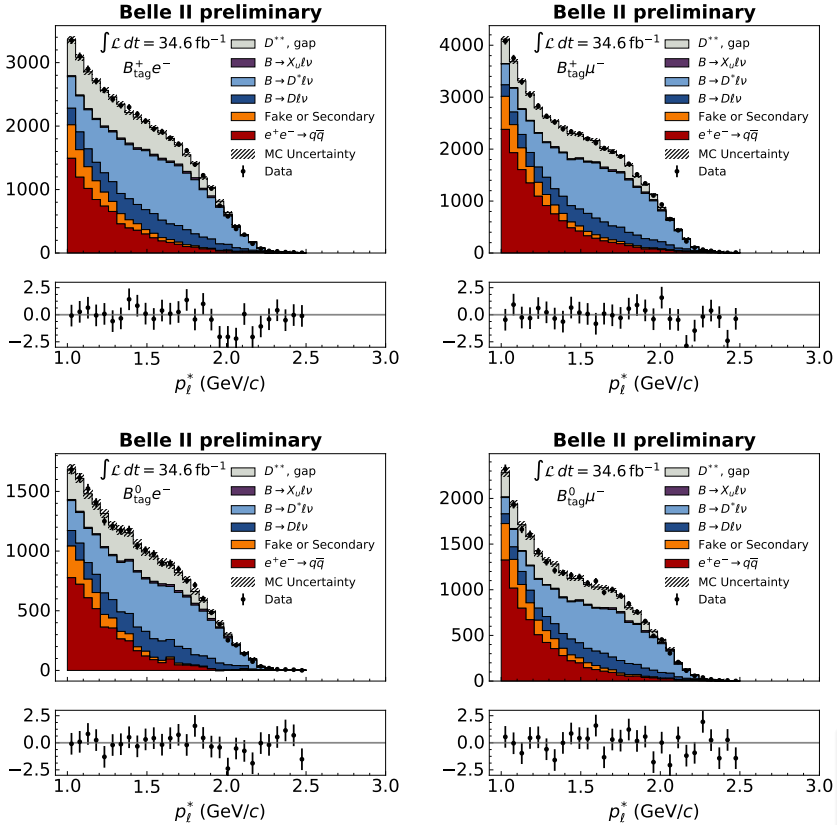
\includegraphics[width=1\textwidth]{figures/data_sim_corrections/tag_calibration.png}
        }
    }
    \caption{\label{fig:fei_calib} Illustration of the fits to \B\to$X_{u,c}\ell\nu$ decays in the \FEI calibration study.
    Results for the combinations of charged and neutral tag-$B$ modes with $e^-$ and $\mu^-$
    are shown in \Cref{fig:fei_calib_bpluseminus,fig:fei_calib_bplusmuminus,fig:fei_calib_bzeroeminus,fig:fei_calib_bzeromuminus}.
    Different fit components are shown in the legend and the subpanels contain the pulls of the fit.
    Figures taken from \cite{Belle-II:2020fst}.
    }
\end{figure}

Branching fractions of $B\rightarrow X_{u,c}\ell\nu$ are evaluated from the fitted distributions.
These values are then directly compared with the experimentally known values of branching fractions of these decays.
A correction factor, $\mathcal{C}_{\mathrm{FEI}}$ is derived, such that the two values are compatible.
The leading evaluated systematic uncertainties are found to be the imperfect experimental knowledge of the $B\rightarrow X_u\ell\nu$ branching fractions and their form factors, the fit model composition, tracking and particle identification uncertainties.
For the Belle II simulation campaign used in this analysis and averaged for both lepton modes, the result is as follows:
\begin{equation}\label{eq:fei_calibration}
    \mathcal{C}_{\mathrm{FEI}}(B^+) = 0.6599 \pm 0.225 \quad \mathcal{C}_{\mathrm{FEI}}(B^0) = 0.6695 \pm 0.0237,
\end{equation}
where two different calibration factors are presented for \feiBp and \feiBz modes, respectively.
Therefore, for an adequate comparison with Belle II data, any Belle II simulation involving the use of \FEI will be henceforth scaled appropriately.

\subsection{Calibration of \texorpdfstring{\piz}{pi0} and \texorpdfstring{$\eta$}{eta} suppression tools}\label{sec:piz_eta_calibration}
It was seen in \Cref{sec:selection_vetos}, that one of the strongest tools for background suppression in this analysis is the $\piz$ and $\eta$ suppression tool.
Consequentially, any data-simulation discrepancies will have a high impact on the final result.
The calibration of the \piz and \eta veto is performed in an independent study and is not part of original work presented in this thesis.
For clarity, the calibration is discussed in this Section. 